\section{Descripción del entorno}
\label{sec:DescripcionEntorno}

Para poder desarrollar la herramienta se han creado unos entornos de pruebas basado en Unreal Engine 5.7.
Son estos entornos los que se van a comunicar con el agente \gls{LLM} de Python.

Estos entornos, de los que se pueden ver un ejemplo en la figura \ref{fig:entorno}, constan de un agente (el \gls{npc} que va a seguir el comportamiento buscado) cuyo controlador es una clase que hereda de la clase de Unreal Engine ``AIController''.
Esta clase contiene los componentes de \gls{BB} y \gls{BT} necesarios para la futura ejecución de un \gls{BT}.
En la misma figura se puede apreciar la interfaz en la que el usuario debe introducir la información necesaria para la generación del \gls{BT}: la descripción del comportamiento buscado, el nombre con el que se va a guardar el \gls{BT} generado, las entradas de la \gls{BB}, el agente que va a ejecutar el \gls{BT} generado y, opcionalmente, el nombre del archivo de validación del \gls{BT} generado.
Esta información la debe contener un actor, llamado en la captura ``BTGeneratorManager'', que tenga un componente llamado ``BTGenerator''.
Este componente de actor es el encargado de lanzar el proceso de Python con la información que el usuario haya puesto, y el que comienza la ejecución de las pruebas del \gls{BT} generado.
Para comenzar la ejecución se debe pulsar el botó ``GenerateBT'' que se aprecia en la captura.

\begin{figure}[H]
    \centering
    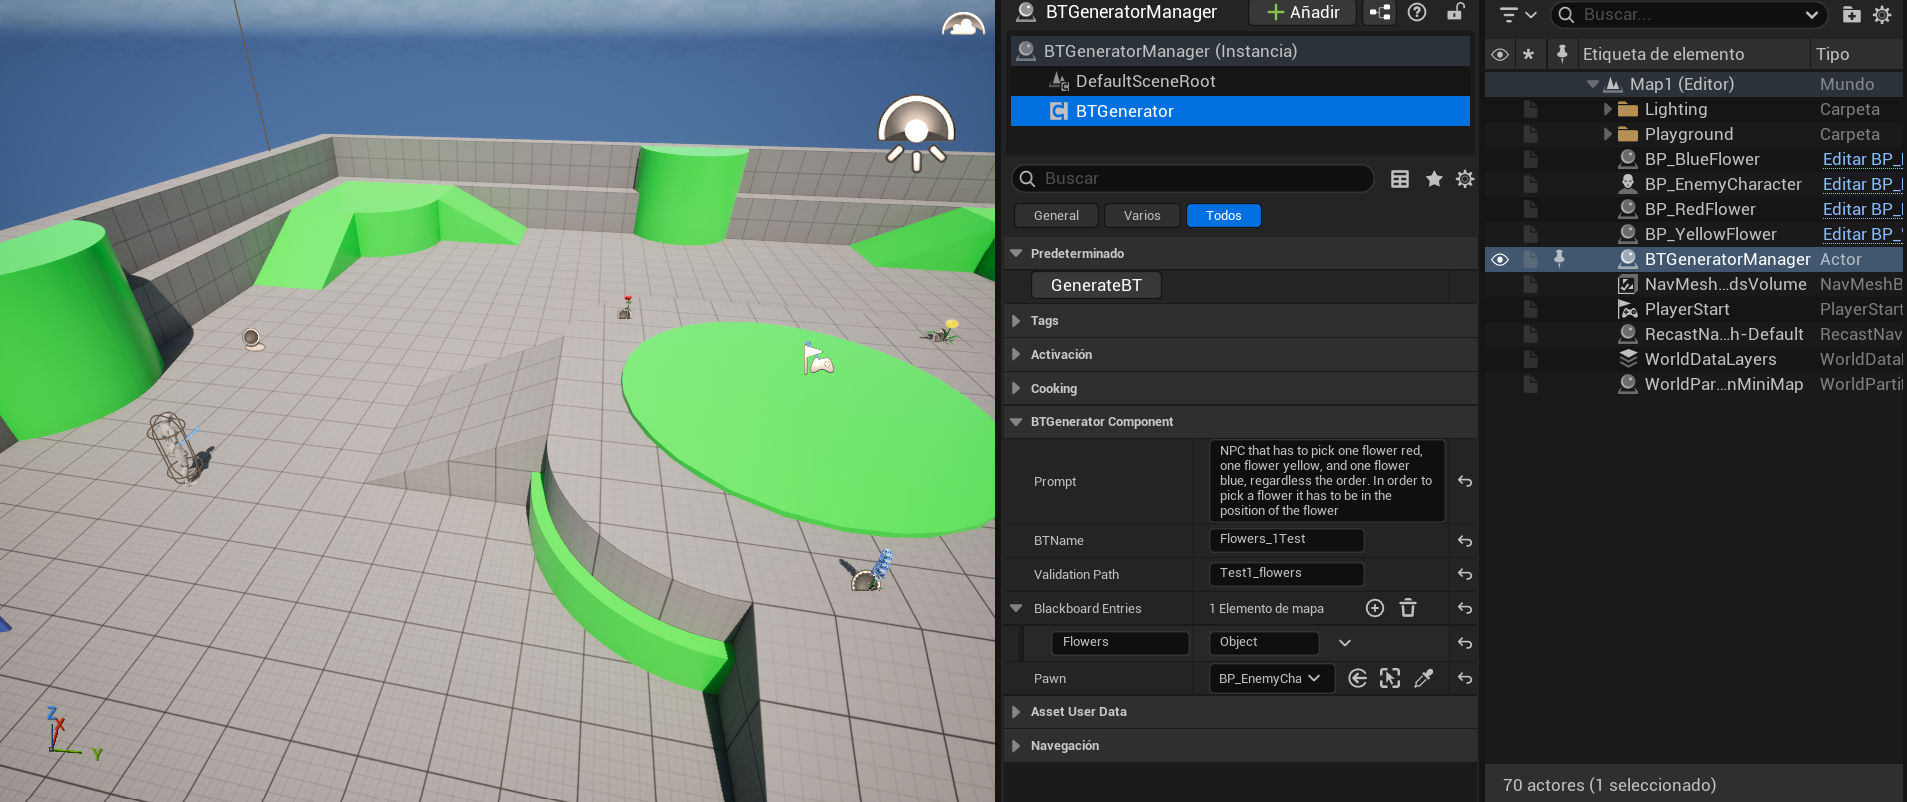
\includegraphics[width=1.0\textwidth]{Imagenes/Bitmap/Entorno1.png}
    \caption[Entorno de desarrollo]{Captura de pantalla de uno de los entornos creados para el desarrollo de la herramienta.}
    \label{fig:entorno}
\end{figure}

Junto con este agente se han preparado una serie de tareas (los cuales servirán como nodos terminales de los árboles) y condicionales que sirven como base para poder crear unos comportamientos de prueba.
Estas tareas y condicionales son introducidos en una clase ``BTFactory'', la cual es un \gls{Abstract Factory} implementado para la construcción de los \glspl{BT}.
Esta clase, la cual se inicializa desde el componente ``BTGeneratorComponent'', contiene tres diccionarios que guardan las tareas, las tareas que necesitan una variable de la \gls{BB} y los condicionales.
Estos diccionarios reciben como clave un string, que es la ID de la tarea o el condicional, y como valor una función (implementada en la propia clase) que crea el objeto que se ha pedido.
Además esta clase tiene otro diccionario que contiene la descripción de cada tarea y condicional, la cual es fundamental para la futura generación de los \glspl{BT}.
Para registrar una nueva clase en esta factoría se debe llamar a las funciones ``RegisterTask'', ``RegisterBlackboardTask'' o ``RegisterDecorator'', las cuales son funciones template en las que se les debe poner la clase que se desea ser introducida y pasar como argumentos el ID que se desee poner y la descripción de lo que realiza la tarea o lo que revisa el condicional.
Además, para las clases que requieran una variable de la \gls{BB} es recomendable introducir qué tipo de variable se requiere.

Las tareas, junto con sus descripciones en español (en el trabajo realizado las descripciones han sido escritas en inglés para respetar el idioma del prompt) que se han creado para estas pruebas son las siguientes:

\begin{itemize}
  \item \texttt{RotateToFaceBBEntry}: Rotar hasta encarar objetivo. El objetivo tiene que ser de tipo ``Objeto''.
  \item \texttt{ChasePlayer}: Perseguir al jugador.
  \item \texttt{MoveTo}: Mover a la posición u objeto de destino. La variable objetivo tiene que ser de tipo ``Objeto'' o ``Vector3''
  \item \texttt{FindRandomPatrol}: Elegir un punto aleatorio del mapa y guardarlo como objetivo.
  \item \texttt{Wait}: No hacer nada.
  \item \texttt{PickRedFlower}: Coger una flor roja.
  \item \texttt{PickBlueFlower}: Coger una flor azul.
  \item \texttt{PickYellowFlower}: Coger una flor amarilla.
  \item \texttt{PickBlackFlower}: Coger una flor negra.
  \item \texttt{ChooseRedFlower}: Elegir una flor roja como objetivo.
  \item \texttt{ChooseBlueFlower}: Elegir una flor azul como objetivo.
  \item \texttt{ChooseYellowFlower}: Elegir una flor amarilla como objetivo.
  \item \texttt{ChooseBlackFlower}: Elegir una flor negra como objetivo.
  \item \texttt{Attack}: Atacar si hay algún objetivo cerca.
  \item \texttt{SelectWaypoint}: Elegir un punto de ruta aleatorio y establecerlo como objetivo. El objetivo debe ser de tipo ``Objeto''
\end{itemize}

Los condicionales implementados, junto con sus descripciones en español (al igual que las tareas, las descripciones en el trabajo están en inglés), son los siguientes:

\begin{itemize}
  \item \texttt{HasLineOfSight?}: Cierto si el jugador está en línea de visión, falso si no. La variable que verifica tiene que ser de tipo ``Bool''
  \item \texttt{IsItNear?}: Cierto si la distancia entre el ejecutor y el jugador es menor o igual que un umbral prefijado, falso en caso contrario. El objetivo tiene que ser de tipo ``Objeto''.
\end{itemize}

Las tareas y condicionales que necesiten una variable de la \gls{BB} necesitan seleccionarla desde el objeto de la \gls{BB} (llamado en Unreal ``BlackboardData'') a través de una variable que tienen los condicionales y las tareas que hereden de la clase de Unreal ``BTTask\_BlackboardBase'', que son las tareas que requieren de una variable.
Sin embargo esta variable es protegida, por lo que se ha creado una interfaz intermedia llamada ``BaseTask'' (de la que heredan todas las tareas que requieran una variable) que contiene las funciones necesarias para acceder a esta variable protegida que permite seleccionar la variable deseada de la \gls{BB}.

El número de terminales y decoradores disponibles en esta implementación es reducido, pero sirve
como sistema de prueba para la generación y la propuesta de evaluación.

Para la generación del JSON se ha seguido una definición de JSON Schema (Draft 2020-12) que delimita la estructura de la generación del JSON para adaptarlo a las necesidades del trabajo.
Este JSON Schema consta de dos partes: el \gls{BB} y el \gls{BT}.
El \gls{BB} es una lista de objetos JSON que contienen solo un par clave-valor, donde la clave es el nombre de la variable y el valor es el tipo de la variable (Bool, Int, Float, Vector, Object o String).
El \gls{BT} consta de un nodo (la raíz) que debe contener el tipo de nodo (Task, Sequence, Selector o Parallel), una lista de decoradores (en el caso de no tener se debe quedar vacía), la cual consiste en objetos JSON que debe contener como clave el nombre del decorador y como valor la varaible de la \gls{BB} que va a usar, y una lista de nodos hijos.
Estos nodos hijos siguen la misma estructura que la raíz.
Como propiedades adicionales, puede contener una lista de nombres de variables de la \gls{BB} que vaya a necesitar, y, en el caso de ser una tarea, debe tener el ID de ésta.
Este esquema se puede encontrar en el apéndice \ref{appendix:Schema}

Para cuando el modelo haya generado el JSON con el \gls{BT}, la clase ``BTGeneratorComponent'' entra en el modo de juego.
Es en este momento donde el \gls{npc}, desde su función ``BeginPlay'' (función de Unreal que es llamada cuando se inicia el juego), coge el nombre del archivo JSON generado para traducirlo a la lógica de Unreal.
Esta traducción la hace la clase ``BTConstructor'', la cual es una clase que sigue el patrón \gls{Singleton} que es inicializada desde la clase ``BTGeneratorComponent''.
Para la traducción se le pasa a la clase el nombre del archivo y el componente de \gls{BB} que debe contener el \gls{npc} mediante el método ``CreateBT''.
Este método crea un \gls{BT} (clase ``BehaviorTree'') y un \gls{BB} (clase ``BlackboardData'') que serán rellenados con la información del JSON.

Lo primero que se traduce es el \gls{BB} gracias al método ``CreateBlackboardAsset'', el cual recorre toda la lista de vaiables para, dependiendo del tipo de ésta, crear un nuevo objeto de Unreal de tipo ``BlackboardkeyType\_XX'' (donde las XX es el tipo de la variable).
Éstas se guardan dentro del campo ``KeyType'' de una variable creada de tipo ``BlackboardEntry'', que será agregada al campo ``Keys'' de la variable de tipo ``BlackboardData''.
Cuando ya se han creado todas las variables de la \gls{BB} se inicializa mediante el método ``InitializeBlackboard'' del componente ``BlackboardComponent''.

Finalmente se crea el \gls{BT} mediante el método recursivo ``CreateNode''.
Inicialmente crea un objeto de tipo ``FBTCompositeChild'' en el que se guardará y devolverá el nodo que se le haya pasado como parámetro (inicialmente el nodo raíz).
Si no es de tipo ``Task'' se crea un objeto de tipo ``BTCompositeNode'', del cual heredan los nodos compuestos (Selector, Sequence y Parallel) para, posteriormente y de forma recursiva, incializar los nodos hijos comprendidos dentro de la lista ``Nodes'' y establecérselos como sus hijos.
Si por el contrario es de tipo ``Task'' se le pide a la clase ``BTFactory'' una nueva instancia de esa tarea (si no existe esta tarea se devuelve un nodo vacío).
Además, si necesita alguna variable de la \gls{BB}, se llama a las funciones necesarias de éstas tareas para establecérsela.
Finalmente, tanto como para las tareas como para los nodos compuestos, se recorren sus decoradores para inicializarse de la misma forma que las tareas: pidiéndole a ``BTFactory'' una instancia de esa clase y estableciendo las variables de la \gls{BB} necesarias.